\section{Liturgia słowa}

\begin{itemize}
	\item po przybyciu do prezbiterium wszyscy (nawet ksiądz \footnote{jak
		      ksiądz ma na sobie dalmatykę to przyklęka, bo pełni funkcje diakona})
	      przyklękamy przy stopniach ołtarza i rozchodzimy się na swoje miejsca:
	      \begin{itemize}
		      \item \ii~ idzie po stopniach do ołtarza
		      \item \cc1 pomaga \ii~ wejść, a potem idzie do kredencji
		      \item \tt~ idzie do kredencji
		      \item \cc3 idzie do chóru
		      \item \ding{63} już stoi przy stojaku
		      \item \cc2 idzie do kredencji
		      \item \aa1 i \aa2 idą do kredencji
		      \item reszta idzie do chóru
	      \end{itemize}
	\item następuje zasypanie przy ołtarzu, po którym \tt~ schodzi i czeka
	      przy stopniach ołtarza
	\item \aa1 podaje Ewangeliarz \cc1, a \cc1 podaje ją \ii~
	\item \ii~ klęka na najwyższym stopniu i odmawia modlitwę
	\item w międzyczasie \cc1 ustawia się na dole obok \tt
	\item \ii~ po skończonej modlitwie do nich dołącza biorąc ze sobą księgę,
	      przyklękają i krótką drogą udają się do Paschału (patrz Rys.
	      \ref{fig:exultet})
	      \begin{figure}[h!]
		      \centering
		      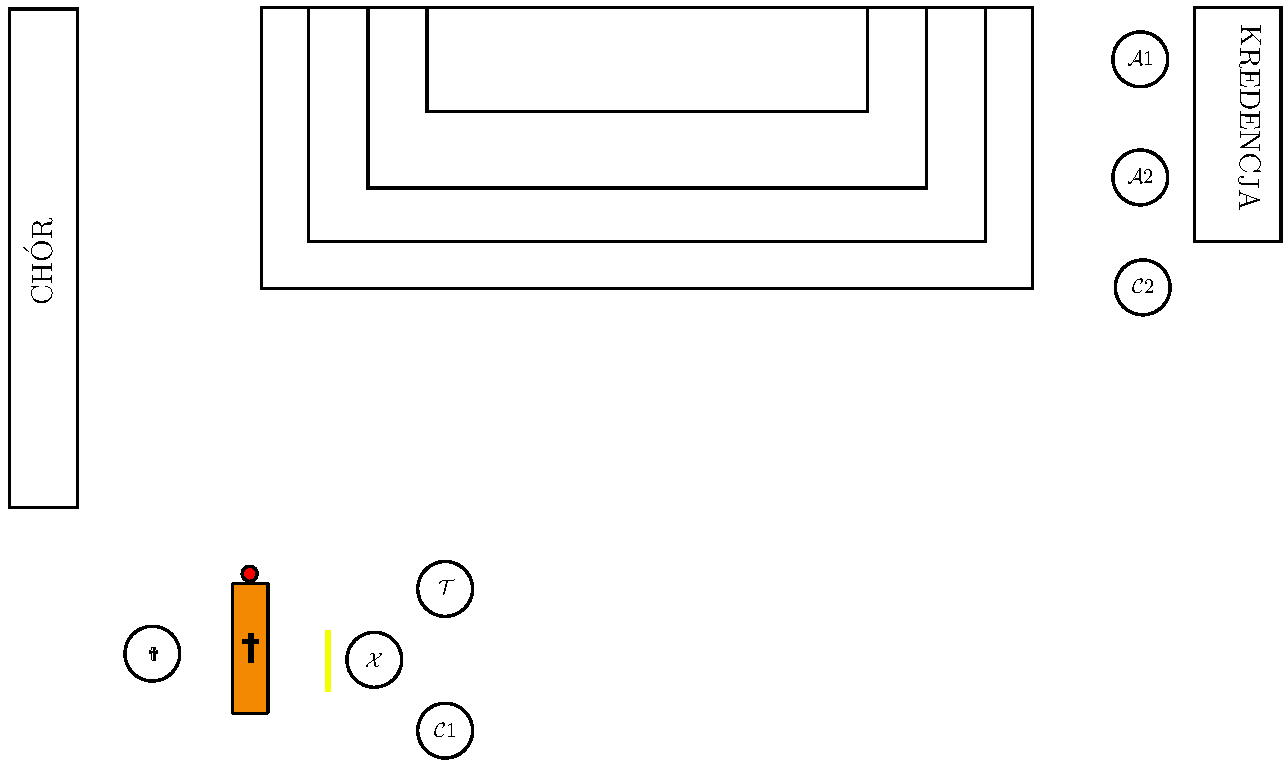
\includegraphics[width=0.8\linewidth]{Figures/Sobota/exultet.pdf}
		      \caption{Exultet}
		      \label{fig:exultet}
	      \end{figure}
	\item następuje okadzenie księgi (3x2), okadzenie Paschału (3x2) i \textit{Exsultet}
	\item \textbf{na śpiew \textit{Exultetu} chór jest zwrócony w stronę Pachału i
		      wszystkie skłony wykonuje do niego}
	\item \aa~ biorą z kredencji świeczki i odpalają sobie
	\item gdyby było odpowiedni ciemno \cc2 na słowa \textit{O vere beata
		      nox...} zapala lampy w prezbiterium.
	\item po orędziu paschalnym \ii, \cc1, \tt~ a za nimi \ding{63} idą na
	      środek ołtarza, klękają (kłaniają się) a następnie \ding{63} idzie
	      odłożyć krzyż, \tt~ idzie na baze a \ii~ z \cc1 udaje się do sedilli,
	      gdzie \cc1 z \cc2 pomagają mu przebrać się w fioletową kapę (kapę
	      przynosi \cc2)
	\item następnie \cc2 odnosi dalmatykę do zakrystii
	\item \zz~ ustawia metalową ambonkę z tekstami proroctw w miejscu, z którego
	      jest normalnie śpiewana lekcja na Mszy
	\item \aa1 kładzie na ołtarzu po stronie Epistoły Mszał
	\item \ii~ z \cc1~ udają się do stopni ołtarza, oddają rewerencje (\cc1~
	      przyklęka a \ii~ wykonuje głęboki skłon), \ii~ wchodzi po stopniach, całuje
	      ołtarz i udaje się do mszału
	\item \ii~ czyta po cichu tekst proroctwa (ewentualnie także kantyku) i, po
	      skłonie do krzyża, krótką drogą udaje się do sedilli
	\item na znak \cc1~ \ii~ wstaje i razem, krótką drogą udaję się do Mszału
	\item \ii~ śpiewa \textit{Oremus} bez skłonu\footnote{bo skłon jest
		      zastępowany przez \textit{Flectamus genua} oraz \textit{Levate}, które także
		      śpiewa \ii}, a potem śpiewa orację
	\item po skończonej oracji czyta po cichu proroctwo i cykl się zamyka
	\item kantorzy śpiewający
	      \begin{itemize}
		      \item jeśli proroctwo poprzedza traktus to podchodzą do ambonki w
		            trakcie jego trwania
		      \item jeśli proroctwa nie poprzedza traktus \footnote{Kantyku nie
			            ma tylko po pierwszym proroctwie} to podchodzą do ambonki pod
		            koniec poprzedzającego proroctwa i stoją z poprzednim kantorem,
		            który odchodzi od ambonki po oracji (stoją obok siebie podczas
		            trwania oracji)
	      \end{itemize}
	\item podczas ostatniego kantyku (\textit{Attende, c\ae lum, et loquar\dots}) \aa\aa~ kładą
	      poduszki na stopniach ołtarza (na środku)
\end{itemize}